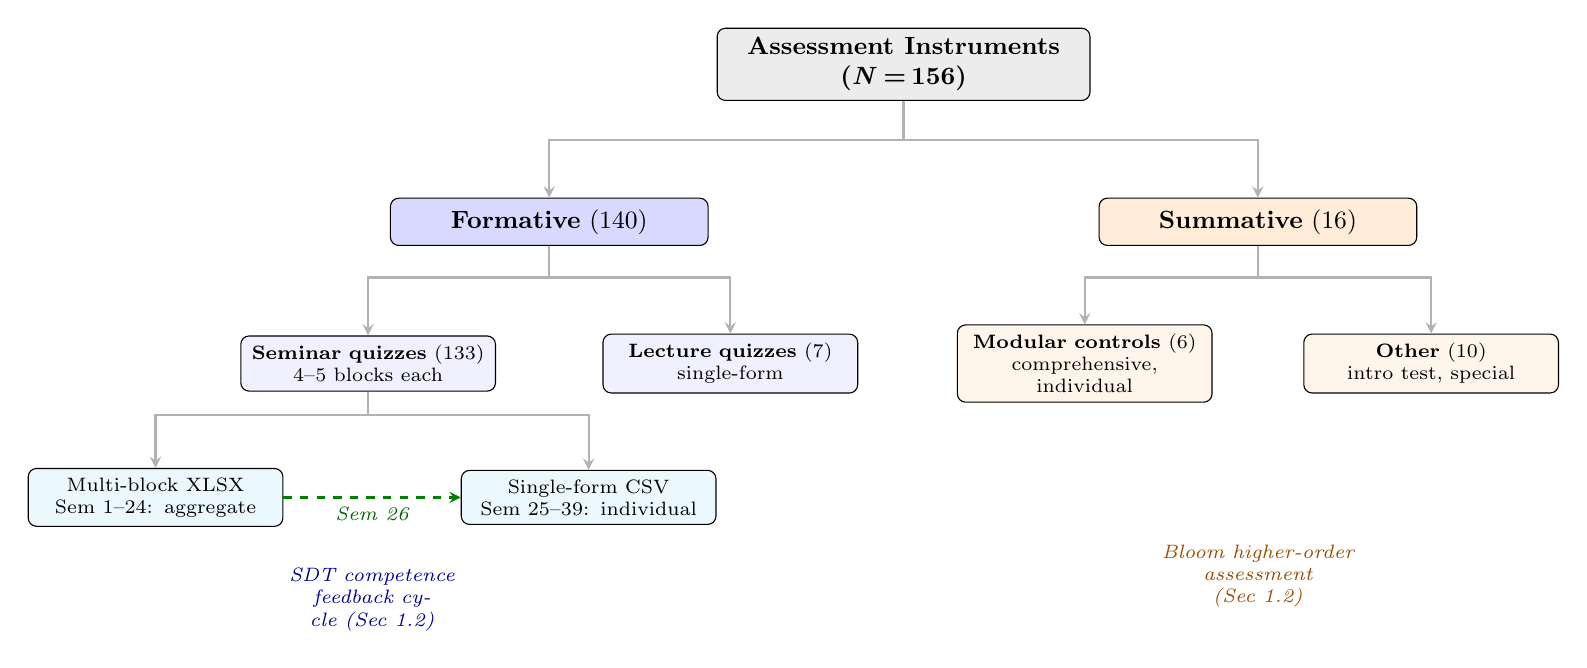
\begin{tikzpicture}[
  node distance=0.45cm,
  rootbox/.style={rectangle, draw, rounded corners=3pt, fill=gray!15,
    text width=4.5cm, minimum height=0.7cm, align=center, font=\small\bfseries},
  formbox/.style={rectangle, draw, rounded corners=3pt, fill=blue!15,
    text width=3.8cm, minimum height=0.6cm, align=center, font=\small},
  summbox/.style={rectangle, draw, rounded corners=3pt, fill=orange!15,
    text width=3.8cm, minimum height=0.6cm, align=center, font=\small},
  leafbox/.style={rectangle, draw, rounded corners=3pt, fill=white,
    text width=3.0cm, minimum height=0.5cm, align=center, font=\scriptsize},
  annot/.style={font=\scriptsize\itshape, text width=2.5cm, align=center},
  arr/.style={->, >=stealth, thick, gray!60}
]

% Root
\node[rootbox] (root) at (0, 0) {Assessment Instruments\\(\textit{N}\,=\,156)};

% Level 1: Formative / Summative — increased vertical gap
\node[formbox] (form) at (-4.5, -2.0) {\textbf{Formative} (140)};
\node[summbox] (summ) at (4.5, -2.0) {\textbf{Summative} (16)};

\draw[arr] (root.south) -- ++(0,-0.5) -| (form.north);
\draw[arr] (root.south) -- ++(0,-0.5) -| (summ.north);

% Formative children — increased vertical gap
\node[leafbox, fill=blue!6] (semq) at (-6.8, -3.8) {\textbf{Seminar quizzes} (133)\\{\scriptsize 4--5 blocks each}};
\node[leafbox, fill=blue!6] (lecq) at (-2.2, -3.8) {\textbf{Lecture quizzes} (7)\\{\scriptsize single-form}};

\draw[arr] (form.south) -- ++(0,-0.4) -| (semq.north);
\draw[arr] (form.south) -- ++(0,-0.4) -| (lecq.north);

% Seminar quiz sub-levels (data format evolution)
\node[leafbox, fill=cyan!8] (xlsx) at (-9.5, -5.5) {Multi-block XLSX\\{\scriptsize Sem 1--24: aggregate}};
\node[leafbox, fill=cyan!8] (csv) at (-4.0, -5.5) {Single-form CSV\\{\scriptsize Sem 25--39: individual}};

\draw[arr] (semq.south) -- ++(0,-0.3) -| (xlsx.north);
\draw[arr] (semq.south) -- ++(0,-0.3) -| (csv.north);

% Transition annotation
\draw[->, >=stealth, thick, green!50!black, dashed] (xlsx.east) -- node[below, font=\scriptsize\itshape, green!40!black] {Sem~26} (csv.west);

% Summative children — increased vertical gap
\node[leafbox, fill=orange!8] (mc) at (2.3, -3.8) {\textbf{Modular controls} (6)\\{\scriptsize comprehensive, individual}};
\node[leafbox, fill=orange!8] (other) at (6.7, -3.8) {\textbf{Other} (10)\\{\scriptsize intro test, special}};

\draw[arr] (summ.south) -- ++(0,-0.4) -| (mc.north);
\draw[arr] (summ.south) -- ++(0,-0.4) -| (other.north);

% Side annotations: placed BELOW the trees
\node[annot, text=blue!60!black] at (-6.75, -6.8) {SDT competence\\feedback cycle (Sec~1.2)};
\node[annot, text=orange!60!black] at (4.5, -6.5) {Bloom higher-order\\assessment (Sec~1.2)};

\end{tikzpicture}
